\documentclass[tikz, border = 10pt]{standalone}

\usepackage{newpxtext,newpxmath}   % /upbeta
%\usepackage{fouriernc}            % /otherbeta
\usepackage{amsmath}
\renewcommand{\familydefault}{\sfdefault}
\usepackage{mathastext}

\usetikzlibrary{positioning, quotes, calc, math, arrows.meta, bending, shapes, backgrounds}

\tikzset{
every edge quotes/.style = {fill = white},
every node/.style = {scale = 1.1},
manifest/.style = {rectangle, draw, thin, inner sep = 3pt, minimum width = 1cm,
   minimum height = .85cm, align = center},
latent/.style = {ellipse, draw, thin, inner sep = 3pt, minimum width = 1cm,
   minimum height = .85cm},
residual1/.style = {circle, draw, thin, minimum size = 5mm, inner sep = 1pt},
residual2/.style = {rectangle, minimum width = 0.5pt, minimum height = 1.5mm,
   inner sep = 0pt, outer sep = 0mm},
regression/.style = {-{Stealth[length = 1.5mm]}, thin, shorten > = 1pt, 
   inner sep = 1.5pt, outer sep = 0mm},
covariance/.style={{Stealth[length = 1.5mm]}-{Stealth[length = 1.5mm]}, thin,
   shorten > = 1pt, shorten < = 1pt, inner sep = 1.5pt},
variance/.style={{Stealth[length = 1mm]}-{Stealth[length = 1mm]}, thin,
   shorten > = 1pt, shorten < = 1pt, inner sep = 1pt},
interaction/.style = {-{Stealth[sep = 1pt, length = 1.5mm] . Circle[length = 4pt]},
   thin, shorten > = -2pt},
constant/.style = {draw, thin, inner sep = 1pt, regular polygon,
   regular polygon sides = 3, minimum size = 5mm},
group/.style = {rectangle, inner sep = 2pt, minimum width = 15mm, minimum height = 5mm, 
   align = center}
}

\begin{document}
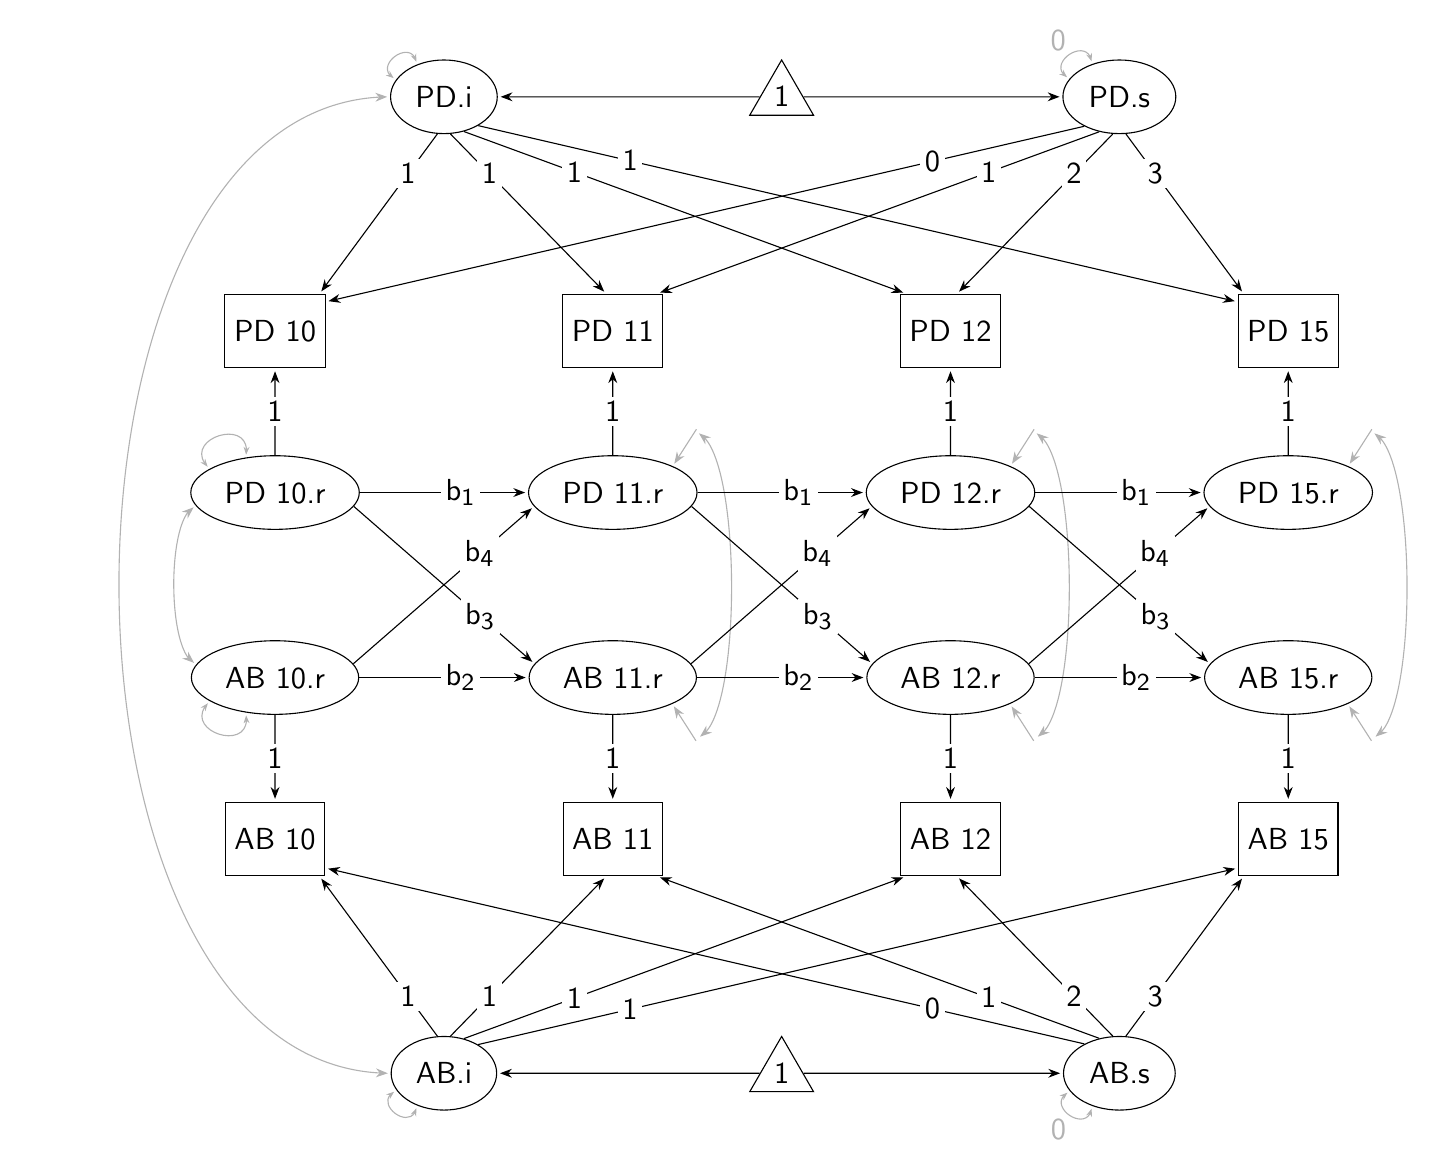
\begin{tikzpicture}

%% The manifest variables
\node [manifest] (x1) {PD 10};
\node [manifest] (x2) [right = 3cm of x1] {PD 11};
\node [manifest] (x3) [right = 3cm of x2] {PD 12};
\node [manifest] (x4) [right = 3cm of x3] {PD 15};

\node [manifest] (y1) [below = 5.5cm of x1] {AB 10};
\node [manifest] (y2) [below = 5.5cm of x2] {AB 11};
\node [manifest] (y3) [below = 5.5cm of x3] {AB 12};
\node [manifest] (y4) [below = 5.5cm of x4] {AB 15};

%% Intercepts and slopes
\coordinate (m1) at ($(x1)!0.5!(x2)$);
\coordinate (m2) at ($(x3)!0.5!(x4)$);
\node [latent] (pdi) [above = 2.5cm of m1] {PD.i};
\node [latent] (pds) [above = 2.5cm of m2] {PD.s};

\path [regression] (pdi.260) edge ["1", pos = 0.25] (x1.40); 
\path [regression] (pdi.280) edge ["1", pos = 0.25] (x2.100); 
\path [regression] (pdi.300) edge ["1", pos = 0.25] (x3.140); 
\path [regression] (pdi.320) edge ["1", pos = 0.2] (x4.150); 

\path [regression] (pds.220) edge ["0", pos = 0.2] (x1.30); 
\path [regression] (pds.240) edge ["1", pos = 0.25] (x2.40); 
\path [regression] (pds.260) edge ["2", pos = 0.25] (x3.80); 
\path [regression] (pds.280) edge ["3", pos = 0.25] (x4.140); 

\coordinate (m3) at ($(y1)!0.5!(y2)$);
\coordinate (m4) at ($(y3)!0.5!(y4)$);
\node [latent] (abi) [below = 2.5cm of m3] {AB.i};
\node [latent] (abs) [below = 2.5cm of m4] {AB.s};

\path [regression] (abi.100) edge ["1", pos = 0.25] (y1.320); 
\path [regression] (abi.80) edge ["1", pos = 0.25] (y2.260); 
\path [regression] (abi.60) edge ["1", pos = 0.25] (y3.220); 
\path [regression] (abi.40) edge ["1", pos = 0.2] (y4.210); 

\path [regression] (abs.140) edge ["0", pos = 0.2] (y1.330); 
\path [regression] (abs.120) edge ["1", pos = 0.25] (y2.320); 
\path [regression] (abs.100) edge ["2", pos = 0.25] (y3.280); 
\path [regression] (abs.80) edge ["3", pos = 0.25] (y4.220); 

%% Their variances - intercept variances freely estimated, slope variances constrained to zero
\path [variance, black!30] (pdi.160) edge [above left, bend left = 120, looseness = 3] (pdi.130);
\path [variance, black!30] (pds.160) edge ["0", above left, bend left = 120, looseness = 3] (pds.130);
\path [variance, black!30] (abi.230) edge [below left, bend left = 120, looseness = 3] (abi.200);
\path [variance, black!30] (abs.230) edge ["0", below left, bend left = 120, looseness = 3] (abs.200);

% Their means
\node [constant] (const1) at ($(pdi)!0.5!(pds)$) {1};
\node [constant] (const2) at ($(abi)!0.5!(abs)$) {1};

\path [regression] (const1) edge [] (pdi); 
\path [regression] (const1) edge [] (pds); 

\path [regression] (const2) edge [] (abi); 
\path [regression] (const2) edge [] (abs); 

%% Intercept covariance
\path [covariance, black!30] (pdi.180) edge [bend right = 90, looseness = 0.95] (abi.180);

%% Structured residuals
\node [latent] (x1r) [below = 1.1cm of x1] {PD 10.r};
\node [latent] (x2r) [below = 1.1cm of x2] {PD 11.r};
\node [latent] (x3r) [below = 1.1cm of x3] {PD 12.r};
\node [latent] (x4r) [below = 1.1cm of x4] {PD 15.r};

\path [regression] (x1r) edge ["1"] (x1);
\path [regression] (x2r) edge ["1"] (x2);
\path [regression] (x3r) edge ["1"] (x3);
\path [regression] (x4r) edge ["1"] (x4);

\node [latent] (y1r) [above = 1.1cm of y1] {AB 10.r};
\node [latent] (y2r) [above = 1.1cm of y2] {AB 11.r};
\node [latent] (y3r) [above = 1.1cm of y3] {AB 12.r};
\node [latent] (y4r) [above = 1.1cm of y4] {AB 15.r};

\path [regression] (y1r) edge ["1"] (y1);
\path [regression] (y2r) edge ["1"] (y2);
\path [regression] (y3r) edge ["1"] (y3);
\path [regression] (y4r) edge ["1"] (y4);

%% Regressions - Stability
\path [regression] (x1r) edge ["$b_{1}$", pos = 0.6] (x2r); 
\path [regression] (x2r) edge ["$b_{1}$", pos = 0.6] (x3r); 
\path [regression] (x3r) edge ["$b_{1}$", pos = 0.6] (x4r); 

\path [regression] (y1r) edge ["$b_{2}$", pos = 0.6] (y2r); 
\path [regression] (y2r) edge ["$b_{2}$", pos = 0.6] (y3r); 
\path [regression] (y3r) edge ["$b_{2}$", pos = 0.6] (y4r); 

%% Regressions - Cross-lagged effects
\path [regression] (x1r.350) edge ["$b_{3}$", pos = 0.7] (y2r.170); 
\path [regression] (x2r.350) edge ["$b_{3}$", pos = 0.7] (y3r.170); 
\path [regression] (x3r.350) edge ["$b_{3}$", pos = 0.7] (y4r.170); 

\path [regression] (y1r.10) edge ["$b_{4}$", pos = 0.7] (x2r.190); 
\path [regression] (y2r.10) edge ["$b_{4}$", pos = 0.7] (x3r.190); 
\path [regression] (y3r.10) edge ["$b_{4}$", pos = 0.7] (x4r.190); 

%% Exogenous variances and covariance
\path [variance, black!30] (x1r.160) edge [bend left = 120, looseness = 3] (x1r.130);
\path [variance, black!30] (y1r.230) edge [bend left = 120, looseness = 3] (y1r.200);
\path [covariance, black!30] (x1r.190) edge [bend right = 80, looseness = 0.5] (y1r.170);

%% Residuals ...
\node [residual2] (e2) [above right = 4mm and 3mm of x2r] {};
\node [residual2] (e3) [above right = 4mm and 3mm of x3r] {};
\node [residual2] (e4) [above right = 4mm and 3mm of x4r] {};
\path [regression, black!30] (e2) edge (x2r.north east);
\path [regression, black!30] (e3) edge (x3r.north east);
\path [regression, black!30] (e4) edge (x4r.north east);

\node [residual2] (e6) [below right = 4mm and 3mm of y2r] {};
\node [residual2] (e7) [below right = 4mm and 3mm of y3r] {};
\node [residual2] (e8) [below right = 4mm and 3mm of y4r] {};
\path [regression, black!30] (e6) edge (y2r.south east);
\path [regression, black!30] (e7) edge (y3r.south east);
\path [regression, black!30] (e8) edge (y4r.south east);

%% and their covariances
\begin{scope}[on background layer]
\path [covariance, black!30] (e2.260) edge [bend left = 75, looseness = 0.4] (e6.80);
\path [covariance, black!30] (e3.260) edge [bend left = 75, looseness = 0.4] (e7.80);
\path [covariance, black!30] (e4.260) edge [bend left = 75, looseness = 0.4] (e8.80);
\end{scope}

\end{tikzpicture}
\end{document}
